\documentclass[../revisedMain.tex]{subfiles}
\begin{document}
	Sometimes none of the aforementioned ways for calculating limits works. One way to calculate possibly impossible limits is the squeeze theorem:
	\begin{quote}
		On an interval containing a point $c$, if $f(x)\leq g(x) \leq h(x)$ for all of the interval, and $\lim\limits_{x\to c} f(x) = \lim\limits_{x\to c} h(x) = a$, then $\lim\limits_{x\to c} g(x) = a$. 
	\end{quote}
	The easiest way to see this is a graph:
		\begin{center}
			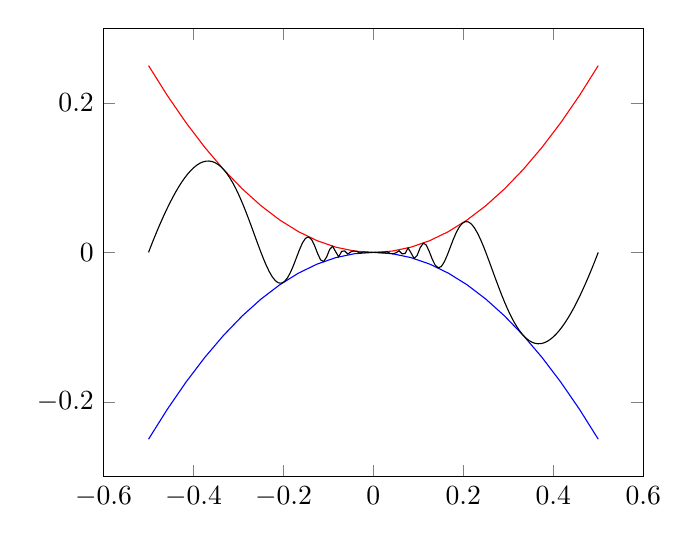
\begin{tikzpicture}
			\begin{axis}
			\addplot[domain=-0.5:0.5, red]{x^2};
			\addplot[domain=-0.5:0.5, blue]{-x^2};
			\addplot[domain=-0.5:0.5, black,samples=150]{x^2*sin(90*x^-1)};
			\end{axis}
			\end{tikzpicture}
		\end{center}
		Here we can see the graph $g(x)=x^2*\text{sin}(\frac{4}{x})$ being squeezed between $f(x)=-x^2$ and $h(x)=x^2$. $g(x)$ has no limit we can compute directly at 0 because $\frac{1}{x}$ has no real limit. However, it is a simple proof to show that $f(x)\leq g(x) \leq h(x)$ and $f(x)$ and $g(x)$ both have the same, real limit for $x=0$, so $$\lim_{x\to 0} f(x) = \lim_{x\to 0} h(x) =\lim_{x\to 0} g(x)= 0$$
\end{document}